\section{Experiments}

\subsection{Training configuration}

\subsection{Comparison to baselines}

\begin{figure}[t]
	\begin{center}
		% \fbox{\rule{0pt}{2in}\rule{0.9\linewidth}{0pt}}
		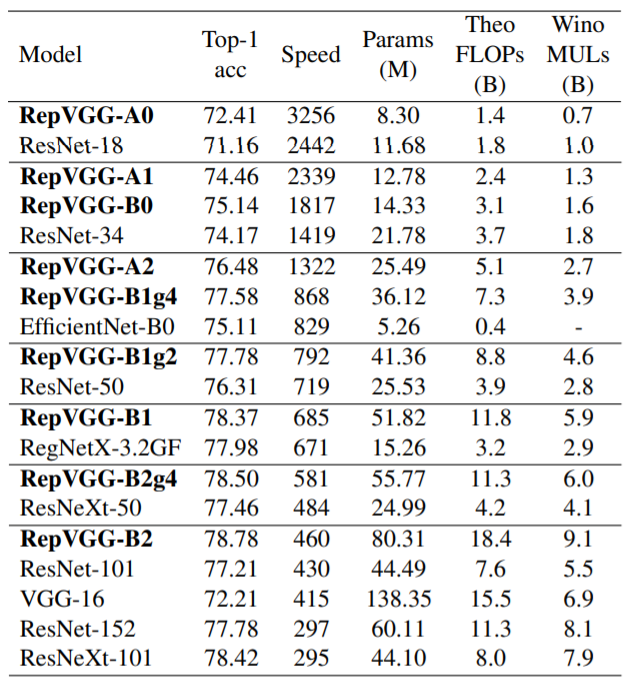
\includegraphics[width=0.8\linewidth]{images/results1.PNG}
	\end{center}
	\caption{RepVGG performance on ImageNet after being trained 120 epochs with simple data augmentation. The speed is measured in examples/second.}
	\label{fig:results1}
\end{figure}

When analyzing the empirical results (see \autoref{fig:results1}) one recognizes the following achievements. 

First the light- and middleweight models of RepVGG-A slightly outperform their ResNet baselines in accuracy, but achieve far higher inference speed. For instance RepVGG-A2 having a comparable amount of parameters to ResNet-50 is only 0.17\% better in accuracy, but therefor 83\% faster. Using interleaved groupwise convolutional layers such increases in speed can further be pushed, e.g. when looking at RepVGG-B1g2 and its counterpart baseline ResNet-152. Achieving the same accuracy RepVGG-B1g2 is a whole 2.66 times faster. 

When looking at the parameter efficiency RepVGG manages to outperfom the historical ResNet and VGG competitors. While achieving the same accuracy RepVGG-B1g2 only needs 69\% of the parameters of ResNet-152. The difference is even higher when comparing RepVGG-A0 to VGG-16 which state a reduction around 94\% of the parameters needed (8.30M compared to 138.35M). Obviously such parameter efficiency gains change when comparing RepVGG to more modern architectures like EfficientNet (14.33M RevVGG-B0 vs. 5.26M EfficientNet-B0) or RegNet (15.26M RegNetX-32.GF vs 41.36M RepVGG-B1g2). As the goal of RepVGG is to gain a good accuracy-speed trade-off while using a plain architecture for inference, such parameter inefficiency are justifiable and difficult to avoid. 

Also it is worth noticing that RepVGG models can of course - at the costs of the amount of parameters needed - keep up with state-of-the-art models. The authors therefore try to make a point by comparing e.g. EfficientNet-B0 to RepVGG-A2 being 1.37\% more accurate and 59\% faster. The question remains whether this can be seen as a valid argument as EfficientNet-B0 uses far less parameters compared to Rep-VGG-A2. If one compares models with approximately equal number of parameters like ResNeXt-50 to RepVGG-A2 such accuracy guarantees will no longer outperform the state-of-the-art models (77.46 vs. 76.48). Nevertheless the speed-up factors remain the strong accomplishment of all RepVGG models (484 ResNeXt-50 vs. 1322 RepVGG-A2). The comparison of ResNeXt-50 and RepVGG-A2 is in addition a perfect proof of the thesis that speed cannot be approximated with FLOPs. If so ResNeXt-50 should have been faster in inference as having less theoretical FLOPs compared to RepVGG-A2 (4.2 vs. 5.1). Winograd multiplications on the other hand seem to work as a better metric to derive speed comparisons (4.1 ResNeXt-50 vs. 2.7 RepVGG-A2). 

\begin{figure}[t]
	\begin{center}
		% \fbox{\rule{0pt}{2in}\rule{0.9\linewidth}{0pt}}
		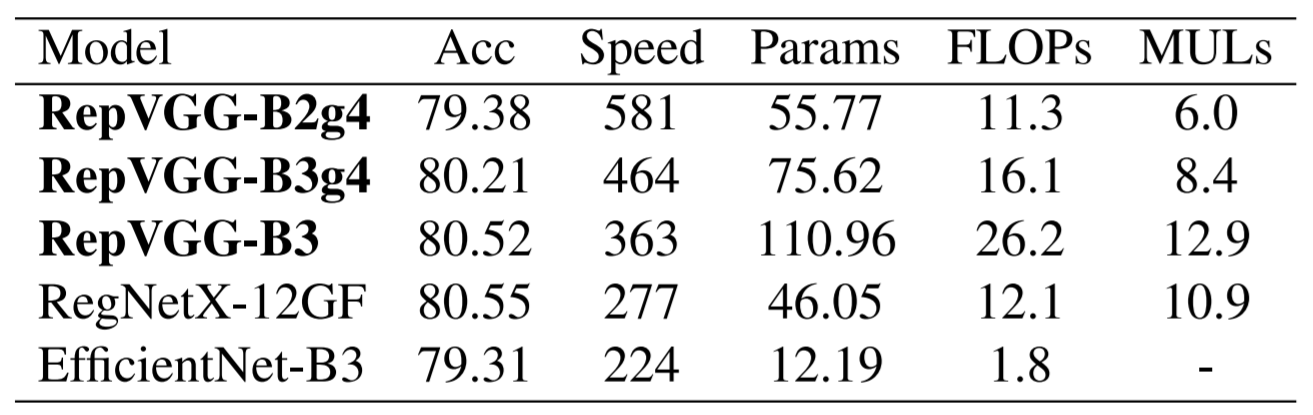
\includegraphics[width=0.8\linewidth]{images/results2.PNG}
	\end{center}
	\caption{RepVGG performance on ImageNet after being trained 200 epochs with Autoaugment, label smoothing and mixup.}
	\label{fig:results2}
\end{figure}

The fact that RepVGG as the first of its kind achieved an accuracy of over 80\% on ImageNet is also not to forget (see \autoref{fig:results2}).



\subsection{Ablation studies}